\documentclass[a4paper]{article}
\usepackage{color}
\usepackage{url}
\usepackage[T2A]{fontenc}
\usepackage[utf8]{inputenc}
\usepackage[english,serbian]{babel}
\usepackage[fixlanguage]{babelbib}
\usepackage[unicode]{hyperref}
\usepackage{placeins}
\usepackage{graphicx}
\usepackage{float}
\usepackage{subcaption}
\usepackage{listings}
\usepackage[justification=centering]{caption}
\usepackage[tableposition = top]{caption}

\hypersetup{colorlinks,citecolor=green,filecolor=green,linkcolor=blue,urlcolor=blue}

\usepackage{listings}

\definecolor{mygreen}{rgb}{0,0.6,0}
\definecolor{mygray}{rgb}{0.5,0.5,0.5}
\definecolor{mymauve}{rgb}{0.58,0,0.82}

\lstset{ 
  backgroundcolor=\color{white},   % choose the background color; you must add \usepackage{color} or \usepackage{xcolor}; should come as last argument
  basicstyle=\scriptsize\ttfamily,        % the size of the fonts that are used for the code
  breakatwhitespace=false,         % sets if automatic breaks should only happen at whitespace
  breaklines=true,                 % sets automatic line breaking
  captionpos=b,                    % sets the caption-position to bottom
  commentstyle=\color{mygreen},    % comment style
  deletekeywords={...},            % if you want to delete keywords from the given language
  escapeinside={\%*}{*)},          % if you want to add LaTeX within your code
  extendedchars=true,              % lets you use non-ASCII characters; for 8-bits encodings only, does not work with UTF-8
  firstnumber=1,                % start line enumeration with line 1000
  frame=single,	                   % adds a frame around the code
  keepspaces=true,                 % keeps spaces in text, useful for keeping indentation of code (possibly needs columns=flexible)
  keywordstyle=\color{blue},       % keyword style
  language=Python,                 % the language of the code
  morekeywords={*,Ulaz,Izlaz,algoritam, dok, god, radi, iz nisu u, sve, ako, je, iz, za, u,vrati},            % if you want to add more keywords to the set
  numbers=left,                    % where to put the line-numbers; possible values are (none, left, right)
  numbersep=5pt,                   % how far the line-numbers are from the code
  numberstyle=\tiny\color{mygray}, % the style that is used for the line-numbers
  rulecolor=\color{black},         % if not set, the frame-color may be changed on line-breaks within not-black text (e.g. comments (green here))
  showspaces=false,                % show spaces everywhere adding particular underscores; it overrides 'showstringspaces'
  showstringspaces=false,          % underline spaces within strings only
  showtabs=false,                  % show tabs within strings adding particular underscores
  stepnumber=1,                    % the step between two line-numbers. If it's 1, each line will be numbered
  stringstyle=\color{mymauve},     % string literal style
  tabsize=2,	                   % sets default tabsize to 2 spaces
  title=\lstname                   % show the filename of files included with \lstinputlisting; also try caption instead of title
}


\title{Tabu pretraga\\ \small{Seminarski rad u okviru kursa\\Metodologija stručnog i naučnog rada\\ Matematički fakultet}}
\author{Krivokuća Mina, Nićković Teodora, Popović Olivera, Zobenica Darinka\\ \href{mailto:mina.krivokuca@gmail.com}{mina.krivokuca@gmail.com}\\ \href{mailto:nickovic97@gmail.com}{nickovic97@gmail.com}\\
\href{mailto:popovic.olivera97@gmail.com}{popovic.olivera97@gmail.com}\\
\href{mailto:darinkazobenica@gmail.com}{darinkazobenica@gmail.com}}
\date{}


\begin{document}
\maketitle


\begin{abstract}
Problem pretrage je jedan od najznačajnijih i duboko izučavanih problema u teoriji računarstva. Algoritmi pretrage služe da dohvate element iz neke strukture podataka, odnosno unapred zadatog domena diskretnih ili kontinualnih vrednosti, tako da zadovoljava unapred zadate kriterijume. Efikasnost određenog algoritma pretrage zavisi od problema sa kojim se suočavamo. U daljem tekstu biće detaljno opisana tabu pretraga, metaheuristički metod koji je baziran na lokalnoj pretrazi. Koraci algoritma će biti razrađeni i približeni čitaocu kroz primere koda i nekoliko primena nad poznatim problemima kojima se bavi računarstvo.
\end{abstract}

\tableofcontents
\newpage

\section{Uvod}
Tabu pretraga je metaheuristika koja spada u algoritme lokalne pretrage, a koristi se za rešavanje problema kombinatorne optimizacije. \cite{glovertutorial} Razvio je Fred Glover u svom naučnom radu na temu celobrojnog programiranja 1986. godine. \cite{eureka} Glover je imao cilj da izbegne zaglavljivanje pretrage u lokalnim minimumima, što je postigao konceptom tabua.\\

Reč tabu potiče iz tonganskog jezika, polinezijskog jezika koji se govori u Kraljevini Tonga. Izvorno reč označava svetinje, koje su u njihovoj kulturi bile zabranjene, nedodirljive, nedozvoljene za korišćenje. Prisvajanjem u engleski se izgubilo značenje svetinje, i reč označava samo zabranu. \cite{tabueth}\\

Tabu pretraga koristi koncept zabranjenih stanja da prevaziđe problem zaglavljivanja u lokalnim optimumima. Naime, ona što održava tzv. tabu listu, tj. listu stanja u kojima je pretraga već bila, te se u njih ne vraća ponovo. Uz to, tabu pretraga dozvoljava poteze koji pogoršavaju vrednost funkcije koju optimizujemo, pod uslovom da boljih dozvoljenih poteza nema. Ta dva koncepta zajedno dozvoljavaju joj da napusti lokalni optimum i nastavi potragu. \cite{tabusearchbook}\\

Pošto tabu pretraga čuva zabranjena stanja, ne može se trivijalno primeniti na kontinualne probleme gde je korak u pretrazi takav da je mala verovatnoća da će pretraga uopšte i pokušati da se vrati u isto stanje. Zbog ovoga, mnogo češća primena je na diskretnim domenima. Međutim, kod kontinualnih problema se problem može diskretizovati, pustiti tabu pretragu da nađe vrednost blisku nekom optimumu, a zatim iz te tačke pustiti neki algoritam pogodan za kontinualnu pretragu, kao što je gradijentni spust. \cite{tabusearchbook}\\

Tabu pretraga se nekad kombinuje sa rasejanom pretragom, čime se dobija hibridna metoda. Ova nova populaciona metoda pretrage se često koristi za rešavanje velikih nelinearnih problema. \cite{scatter}\\

Cilj ovog rada je da čitaocu približi osnovne koncepte vezane za tabu pretragu na način koji je zanimljiv, edukativan, i precizan. Nakon definicije i objašnjenja osnovnih koncepata i njihove motivacije, izlažemo primere primene tabu pretrage na neke od poznatih NP problema, kao i zaključke iz drugih radova o kvalitetu primene ove metaheuristike u praksi.


\section{Osnovni pojmovi i opis algoritma}

Zadat je sledeći problem kombinatorne optimizacije, konkretno minimizacije funkcije $f$:

$$\min\limits_{x\in X} f(x)$$

Funkcija $f$ ovde može biti linearna ili nelinearna, a skup $X$ predstavlja prostor dopustivih rešenja, i on mora biti konačan \cite{yugobrief}.

Svako $x\in X$ ima svoj skup $N(x)\subset X$, $x\notin N(x)$, i taj skup nazivamo \textbf{okolina} (eng. \textit{neighborhood}) tačke $x$. $N(x)$ je definisan kao skup svih $y\in X$ koje se mogu dobiti direktno na osnovu $x$ modifikacijom koju nazivamo \textbf{pomeraj iz x u y} (eng. \textit{move}) i obeležavamo $m(x,y)$. Rešenje iz okruženja obeležavaćemo sa $x'$. \cite{yugobrief}\\

Jedno od mogućih rešenja ovog problema minimizacije je korišćenje pohlepne pretrage. \cite{vi} Takvo rešenje bilo bi jednostavno za implementaciju i često efikasno za izvršavanje. Međutim, ako se u svakom koraku bira najbolja raspoloživa akcija, takav algoritam će se često zaglavljivati u lokalnim minimumima, a u slučaju platoa se neće zaustavljati bez dodatnih ograničenja. Jedan od načina sprečavanja zaglavljivanja u lokalnom minimumu jeste uvođenje \textbf{tabu liste} (eng. \textit{tabu list}).

\subsection{Tabu lista i kratkoročna memorija}
Tabu lista je lista \textbf{tabu čvorova} (stanja, konfiguracija, poteza...). Glavna ideja tabu liste je da čuva čvorove koji su posećeni, kako se tokom pretrage ne bismo vraćali na ono što je već istraženo \cite{edelkamp}. Tabu čvorovi su oni čvorovi koji se ne mogu posetiti, čak i ako su u trenutnoj okolini $N(x)$. \textbf{Izmenjena okolina} (eng. \textit{modified neighborhood}) $N^*(x)$ je rezultat ovoga, i ona čini skup dopustivih pomeraja. Izmenjena okolina $N^*(x)$ se u ovom slučaju formira kao $N(x)\setminus T$, gde $T$ predstavlja tabu listu. Potom se iz nje bira sledeći korak $x'$. \cite{tabusearchbook}\\

\begin{lstlisting}
Ulaz: Konfiguracija pocetno_resenje
      Int max_iteracija
Izlaz: Konfiguracija najbolje_resenje

algoritam TabuPretraga:
    trenutno_resenje = pocetno_resenje
    najbolje_resenje = pocetno_resenje    
    tabu_lista = [trenutno_resenje]
    za k = 1 do max_iteracija: 
        ako je validno_resenje(trenutno_resenje) i 
                f(trenutno_resenje) < f(najbolje_resenje):
            najbolje_resenje = trenutno_resenje;
        
        tabu_lista.dodaj(trenutno_resenje)
        okolina = generisi_okolinu(trenunto_resenje)
        izmenjena_okolina = [sve konfiguracije iz okoline 
                            koje nisu u tabu listi]
        trenutno_resenje = 
            selektuj_najbolje_ocenjeno_resenje(izmenjena_okolina);

    vrati najbolje_resenje
\end{lstlisting}

Prvi problem sa ovako koncipiranom tabu listom je to što je čuvanje svih obrađenih stanja jako skupo.\cite{coursera} Rešenje koje se nameće je čuvanje samo određenih čvorova koji su nam relevantni, što može biti poslednjih $k$ čvorova. Ovakvo rešenje ima smisla, jer je malo verovatno da će čvorovi koji su davno posećeni uopšte biti u trenutnoj okolini. Ovakva tabu lista naziva se \textbf{kratkoročna memorija}.\cite{tabusearchbook}

Dužina liste u praksi može biti dinamički menjana, tako da s jedne strane spreči zaglavljivanje u lokalnom minimumu, a s druge ne uspori pretragu previše jer svaki potez moraju da se proveravaju svi elementi tabu liste. U nastavku ćemo smatrati da je dužina ove liste fiksna.

Drugi problem na koji nailazimo je da ovakvo čuvanje obrađenih stanja i dalje može biti skupo za neke probleme.\cite{coursera} Razmatrana stanja mogu biti kompleksne konfiguracije koje su memorijski zahtevne za čuvanje, kao i za međusobno poređenje sa razmatranim stanjem u svakoj iteraciji. Zato se tabu lista često implementira tako da čuva neke apstrakcije skupa čvorova koji su skoro posećeni, na primer neke njihve osobine, ili pomeraje koji su nas doveli iz prethodnih stanja u tekuće. Ideja je da se takvi pomeraji ne prave opet, kako ne bismo ponovo došli u stanje sa lošijom vrednošću funkcije.

Ovakva implementacija tabu liste jasnija je na primerima primene. U rešavanju problema putujućeg trgovca, od početne konfiguracije [A, B, C, D, E], možemo dobiti novu tako što zamenimo gradove B i D, i dobijemo [A, D, C, B, E]. Ukoliko je ova konfiguracija lošija od početne, zamena gradova B i D će biti dodata u tabu listu.

\subsection{Kriterijum aspiracije}
U situaciji kada u tabu listi čuvamo pomeraje, a ne cela stanja, može se desiti da je za jednu konfiguraciju određen pomeraj loš, zbog čega on završava u tabu listi, ali da za drugu konfiguraciju on vodi u stanje sa boljom vrednošću funkcije. Drugim rečima, može se desiti da postoji pomeraj koji je tabu, ali u isto vreme i jako dobar. Zbog takvih situacija definišemo  \textbf{kriterijum aspiracije} (eng. \textit{aspiration criteria}). On modifikuje okolinu tako da izmenjena okolina sadrži i pomeraje koji su tabu, ali zadovoljavaju kriterijum aspiracije. Takav kriterijum se može definisati na mnogo načina, od čega je najjednostavniji - da li ovim pomerajem dobijamo konfiguraciju za koju je vrednost funkcije bolja od trenutne?

\subsection{Dugoročna i srednjeročna memorija}
Kratkoročna memorija je sama po sebi često dovoljna za postizanje rezultata koji su bolji od onih postignutih drugim metodama lokalne pretrage \cite{shortonly}. Međutim, često je potrebno pretragu dodatno usmeriti \cite{glovertutorial}. Usmeravanje se može izvršiti na dva načina:

\begin{itemize}
    \item usmeravanje ka regijama koje su obećavajuće
    \item usmeravanje ka neistraženim delovima
\end{itemize}

U slučaju kada pretragu usmeravamo ka obećavajućim regijama, koristimo \textbf{pravila pojačavanja} (eng. \textit{intensification rules}). Takva pravila mogu biti davanje prioriteta nekim karakteristikama dobre ciljne konfiguracije, na primer dobre vrednosti određenih promenljivih ili određenih segmenata konfiguracije. Struktura u kojoj se čuvaju takve karakteristike se naziva \textbf{srednjeročna memorija} (eng. \textit{intermediate-term memory}).


Kada se pretraga usmerava ka neistraženim regijama, koriste se \textbf{pravila diverzifikacije} (eng. \textit{diversification rules}). Ova pravila se koriste u slučaju stagniranja pretrage, kada se ona mora resetovati. Jedan od načina da se ovo postigne je čuvanje konfiguracija koje su u ranijim iteracijama davale dobre rezultate, te se u slučaju stagnacije pretraga vraća na neku od njih. Struktura u kojoj se čuvaju takve konfiguracije se naziva \textbf{dugoročna memorija} (eng. \textit{long-term memory}).
 Važi da je $N^*(x)\subset N(x)$ kod strategija baziranih na kratkoročnoj memoriji, ali ne nužno kod strategija baziranih na dugoročnoj. \cite{tabusearchbook}\\

\section{Primena}
Tabu pretraga je postigla dobre rezultate na širokom dijapazonu problema, koji je dodatno proširen kada se ona ukombinuje sa drugim algoritmima i tehnikama optimizacije. Uspešno rešava kombinatorne, kao i probleme optimizacije nad neprekidnim domenom. \cite{yugobrief} U daljem tekstu ćemo prikazati primenu ovog algoritma na dva tipa problema:
\begin{itemize}
    \item Kombinatorni problemi - \textbf{problem N-dama} (eng. \textit{N-queens problem})
    \item Celobrojno programiranje - \textbf{problem rasporeda objekata sa ograničenim resursima} (eng. \textit{capacitated facility location problem})
\end{itemize}

\subsection{Primena tabu pretrage na problem N-dama}
Treba rasporediti N dama na šahovskoj tabli dimenzije NxN, tako da se nikoje dve međusobno ne napadaju. Početna konfiguracija ovde može biti nasumičan raspored N dama, tako da je na svakoj vertikali tačno jedna. Pomeraj ćemo definisati kao pomeranje dame po svojoj vertikali, na poziciju različitu od trenutne. Cilj pomeraja će biti da se maksimalno smanji broj prekršaja koji postoje u toj konfiguraciji. Dakle, pomeraj je dodeljivanje vrednosti polja jednoj od dama, i jedan pomeraj ćemo zapisivati kao par (dama, polje). Broj prekršaja za jednu konfiguraciju je broj dama koje se međusobno napadaju. Okolinu za svaku damu čine svi njeni mogući pomeraji. U tabu listi čuvaćemo $k$ prethodnih pomeraja, tj. $k$ vrednosti (dama, polje), gde ovi parovi predstavljaju prethodne pozicije odgovarajućih dama. Time ćemo sprečiti da dama ponovo dođe na poziciju na kojoj je već bila.

\begin{lstlisting}
Ulaz: Konfiguracija pocetna_konfiguracija
      Int max_iteracija
      Int max_duzina_tabu_list
Izlaz: Konfiguracija najbolja_konfiguracija

algoritam TabuPretraga:
    trenutna_konfiguracija = pocetna_konfiguracija
    najbolja_konfiguracija = pocetna_konfiguracija
    br_iteracija = 0
    tabu_lista = []
    
    dok god br_iteracija < max_iteracija i
            broj_prekrsaja(trenutna_konfiguracija) > 0 radi:
        okolina = generisi_okolinu(trenutna_konfiguracija)
        izmenjena_okolina = [sve konfiguracije iz okoline 
                            koje nisu u tabu listi]
        ako je duzina(izmenjena_okolina) > 0:
            (dama, novo_polje) = selektuj_najbolji_potez(izmenjena_okolina)
            tabu_lista.dodaj((dama, staro_polje) iz trenutna_konfiguracija)
            zameni vrednost za dama u trenutna_konfiguracija
            
        ako je broj_prekrsaja(trenutna_konfiguracija) 
               < broj_prekrsaja(najbolja_konfiguracija):
            najbolja_konfiguracija = trenutna_konfiguracija
        
        ako je duzina(tabu_lista) >= max_duzina_tabu_liste:
            izbaci_prvi_dodati_element(tabu_lista)
            
        brojac += 1
    
    vrati najbolja_konfiguracija
\end{lstlisting}

Ovo je osnovni oblik algoritma tabu pretrage, primenjen na problem N-dama. Prikazana je samo kratkotočna memorija. U slučaju da želimo da dodamo kriterijum aspiracije, to možemo učiniti na sledeći način.

\begin{lstlisting}
    okolina = generisi_okolinu(trenutna_konfiguracija)
    izmenjena_okolina = [potez iz okolina koji nije u tabu listi ili 
                    broj_prekrsaja(najbolja_konfiguracija) >
                    broj_prekrsaja(trenutna_konfiguracija + potez)]
\end{lstlisting}

Moguće je dodati i dugoročnu memoriju, tako što pamtimo konfiguracije sa malo prekršaja, na koje se možemo vraćati nakon određenog broja iteracija ili male promene u poboljšanju, i time restartovati pretragu od tog trenutka. Implementacija ovog problema u programskom jeziku Python priložena je uz rad. U ovoj konkretnoj implementaciji, dovoljna diverzifikacija je bila resetovanje pretrage i traženje optimalnog rešenja nad svim iteracijama. Parametri za broj resetovanja, broj iteracija svake pretrage i dužinu tabu liste određeni su eksperimentalno, kompletni rezultati se mogu naći u dodatku \ref{appendix:a}.  Neki od najboljih rezultata prikazani su u tabeli \ref{tab:dame}.\\

\begin{center}
\begin{table}[h]
\caption[long]{Testirane kombinacije parametara koje su se dobro pokazale i odgovarajuće vreme}
\label{tab:dame}

\begin{tabular}{| c c c |}
 \hline
 Maksimalni broj iteracija & Dužina tabu liste & Prosečno vreme za N=20 (\textit{s}) \\ 
 \hline
 60 & 11 & 0.637598 \\  
 90 & 16 & 0.770418 \\  
 80 & 16 & 0.805036 \\ 
 50 & 16 & 0.961352 \\ 
 90 & 6  & 1.001105 \\ 
 70 & 6  & 1.090587 \\ 
 90 & 11 & 1.108473 \\ 
 70 & 21 & 1.135153 \\ 
 50 & 11 & 1.187593 \\ 
 \hline
\end{tabular}
\end{table}
\end{center}

\subsection{Primena tabu pretrage na CFLP}
U svom najjednostavnijem obliku, \textbf{problem rasporeda objekata} (eng. \textit{facility location problem - FLP}) je problem nalaženja tačke na ravni, takve da je suma rastojanja od ove tačke do N ciljnih tačaka najmanja (\textbf{Veberov problem}) \cite{weber}. Kompleksije varijante ovog problema bave se postavljanjem više objekata, zadovoljavanjem ograničenja oko njihovih lokacija (npr. radioaktivni objekti ne smeju biti blizu naseljenih mesta) i optimizacijom dodatnih kriterijuma (npr. blizina konkurentnih objekata).\\

Jedno od mogućih ograničenja može biti količina resursa u objektima za skladištenje koji treba da snabdevaju prodajne objekte. To je baš ono čime se bavi \textbf{problem rasporeda objekata sa ograničenim resursima} (eng. \textit{capacitated facility location problem}). Formulacija problema je sledeća: pretpostavimo da imamo M mogućih lokacija za magacine i P prodavnica koje treba snabdevati robom. Za svaku od potencijalnih lokacija magacina poznat je njen kapacitet, kao i cena otvaranja. Za svaku od prodavnica, poznate su njene potrebe, kao i cena transporta robe od svakog od magacina (u rešavanju ovog problema, kao cenu smo uzeli Euklidsko rastojanje prodavnice i magacina). Potrebno je odrediti:
\begin{itemize}
    \item koje magacine otvoriti,
    \item koja prodavnica će se snabdevati iz kog magacina.,
\end{itemize}
tako da robni zahtevi svih prodavnica budu ispunjeni, kao ukupna cena otvaranja magacina i transporta bude minimalna. Dakle, ciljna funkcija nam je ukupna cena, i nju treba minimizovati, uz dodatno zadovoljavanje ograničenja o resursima.

Magacini i prodavnice zovu se po indeksima. U listama su date odgovarajuće karakteristike lokacije, za lokaciju pod tim indeksom. Algoritam vraća najbolju dostignutu vrednosti ciljne funkcije (minimalni trošak), kao i najbolje rešenje, koje je dato listom istinitosnih vrednosti, koje označavaju da li se magacin sa tim indeksom otvara ili ne.

\begin{lstlisting}
Ulaz: Int broj_magacina
      Lista<Int> kapaciteti_magacina
      Lista<Int> cene_otvaranja
      Int broj_prodavnica
      Lista<Int> robni_zahtevi
      Lista<Lista<Float>> cene_transporta
      Int max_iteracija
      Int max_duzina_tabu_liste
      Lista<Bool> pocetno_resenje
Izlaz: Float minimalni_trosak
       Lista<Bool> najbolje_resenje

algoritam TabuPretraga:
    trenutno_resenje = pocetno_resenje
    trenutni_trosak = odredi_vrednost_ciljne_funkcije(svi argumenti
    samog algoritma, sem max_iteracija i max_duzina tabu_liste)
    najbolje_resenje = trenutno_resenje
    minimalni_trosak = trenutni_trosak
    
    br_iteracija = 0
    tabu_lista = [trenutno_resenje]
    
    dok god br_iteracija < max_iteracija:
        okolina = [resenja dobijena invertovanjem tacno jedne istinitosne
                    vrednosti u trenutno_resenje]
        izmenjena_okolina = [svako resenje iz okolina koje ne pripada 
                            tabu listi]
        
        novo_resenje, izmenjeni_magacin =
            odaberi_nasumicno_validno_resenje_iz_izmenjene_okoline()
        
        novi_trosak = izracunaj_vrednost_ciljne_funkcije(svi argumenti
            samog algoritma, sem max_iteracija i max_duzina tabu_liste,
            trenutno_resenje)
        tabu_lista.dodaj(novo_resenje)
        
        // Ukoliko nasumicna izmena pogorsava trosak, ignorisemo je
        // u potpunosti. Time je niz ocena koji se stvara uvek rastuci.
        ako novi_trosak < trenutni_trosak:
            trenutni_trosak = novi_trosak
            trenutno_resenje = novo_resenje
        
        ako trenutni_trosak < minimalni_trosak:
            minimalni_trosak = trenutni_trosak
            najbolje_resenje = trenutno_resenje
        
        ako duzina(tabu_lista) > max_duzina_tabu_liste:
           izbaci_prvi_dodati_element(tabu_lista)
            
    vrati minimalni_trosak, najbolje_resenje
\end{lstlisting}

Direktna implementacija ovog pseudokoda je uvek uspevala da poboljša početno rešenje, međutim često je bila jako neefikasna, i rešenja nisu mnogo napredovala. Diverzifikacija nije mnogo pomogla, kao ni podešavanje parametara dužine tabu liste i broja iteracija. Međutim, uvođenje unutrašnje i spoljašnje petlje je značajno poboljšalo rezultate \cite{loops}. 

Vizuelizacija rešenja nalazi se na slikama \ref{fig:sl1}, \ref{fig:sl2}, i \ref{fig:sl3}. Primeri su generisani sa sledećim osobinama:
\begin{itemize}
    \item zadaje se broj magacina i broj prodavnica
    \item lokacije magacina i prodavnica se generišu nasumično na mapi
    \item zadaje se kapacitet magacina, koji je isti za sve
    \item zadaje cena za otvaranje magacina u centru grada (skuplje), i cena za otvaranje inače (pod centrom grada smatra se unutrašnja četvrtina mapre)
    \item potrebe prodavnica se nasumično generišu nad prethodno zadatim intervalom
    \item cena transporta od magacina do prodavnice je Euklidsko rastojanje između njihovih lokacija
\end{itemize}

Na levoj strani prikazane su prodavnice (crna kolica) i moguće lokacije za magacine (crveni upitnik), a na desnoj lokacije magacina koji će biti otvoreni, dobijene primenom algoritma. Karakteristike svakog od test primera navedene su ispod slike.

\begin{figure}[H]
\centering
\begin{subfigure}{.5\textwidth}
    \centering
    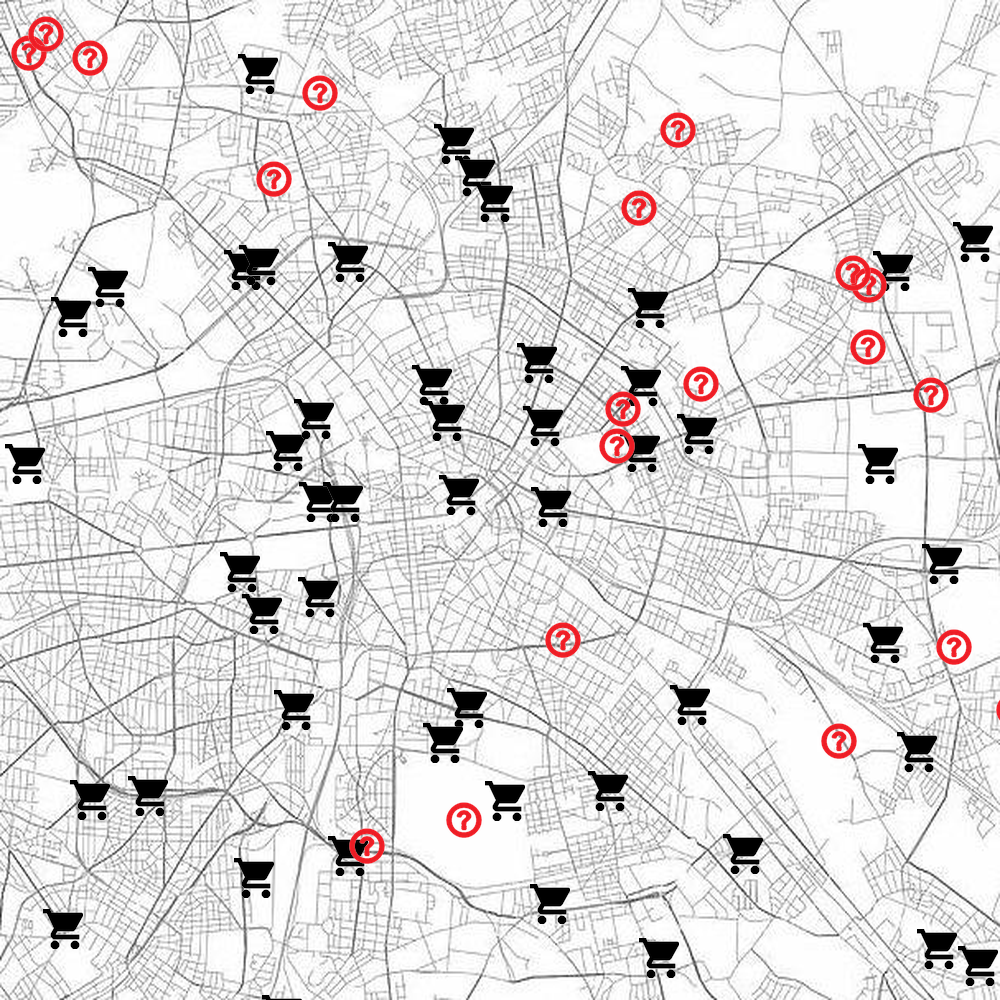
\includegraphics[width=0.95\textwidth]{pics/candidates1.png}
\end{subfigure}%
\begin{subfigure}{.5\textwidth}
    \centering
    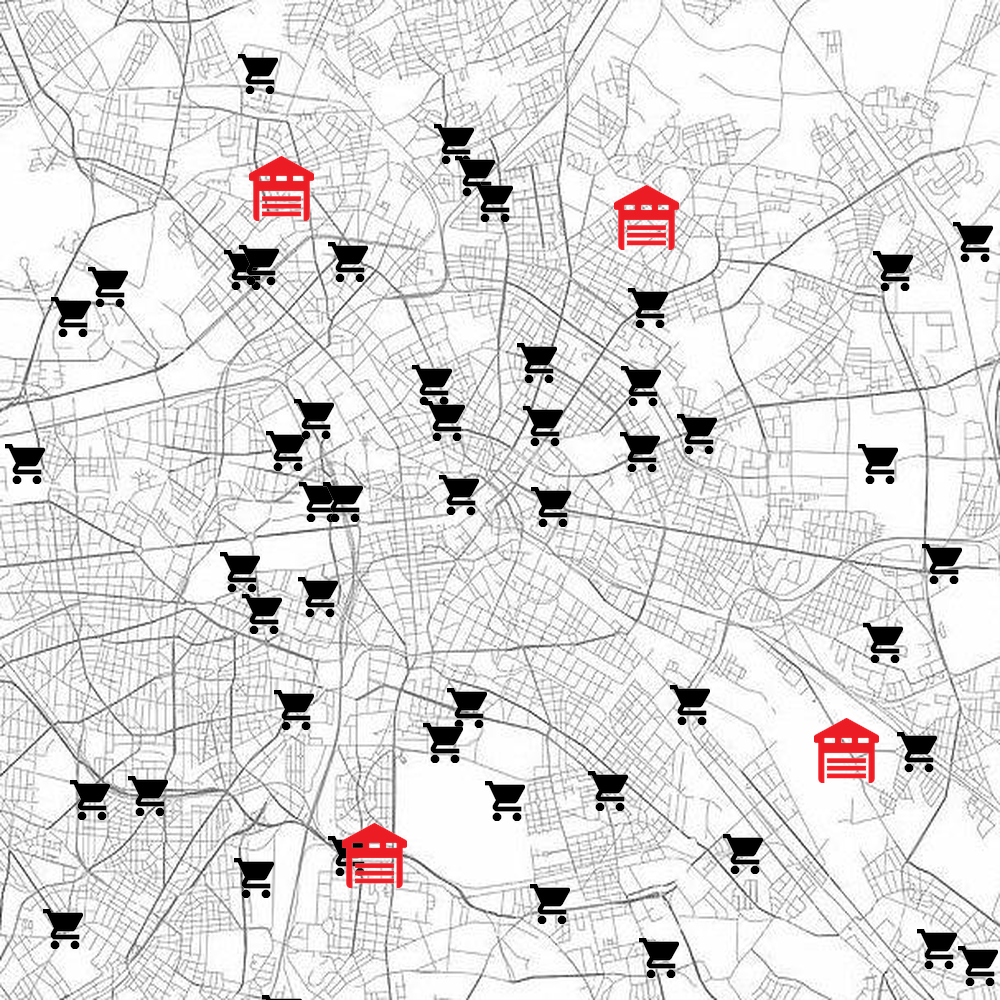
\includegraphics[width=0.95\textwidth]{pics/final1.png}
\end{subfigure}
\caption[long]{Br. magacina: 20, br. prodavnica: 50,\\ cena u centru: 2000, cena inače: 1000}
\label{fig:sl1}
\end{figure}

\begin{figure}[H]
\centering
\begin{subfigure}{.5\textwidth}
    \centering
    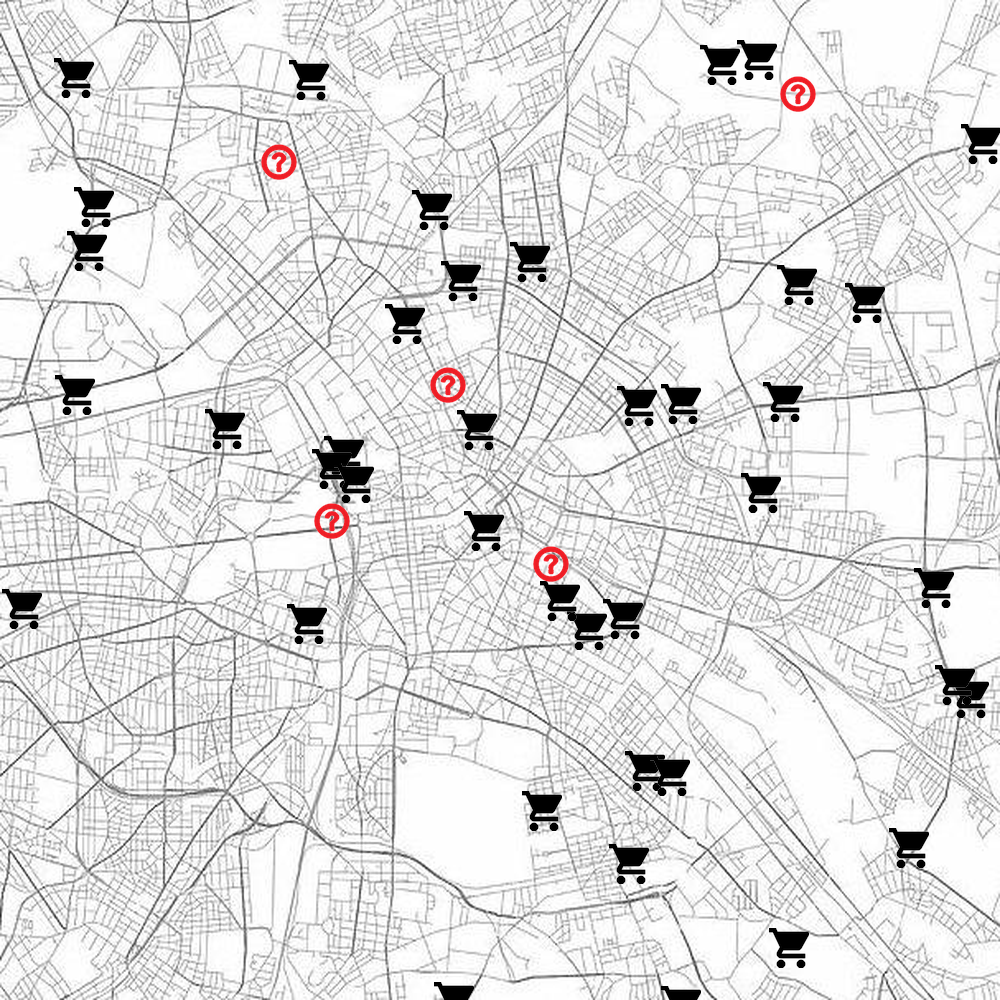
\includegraphics[width=0.95\textwidth]{pics/candidates2.png}
\end{subfigure}%
\begin{subfigure}{.5\textwidth}
    \centering
    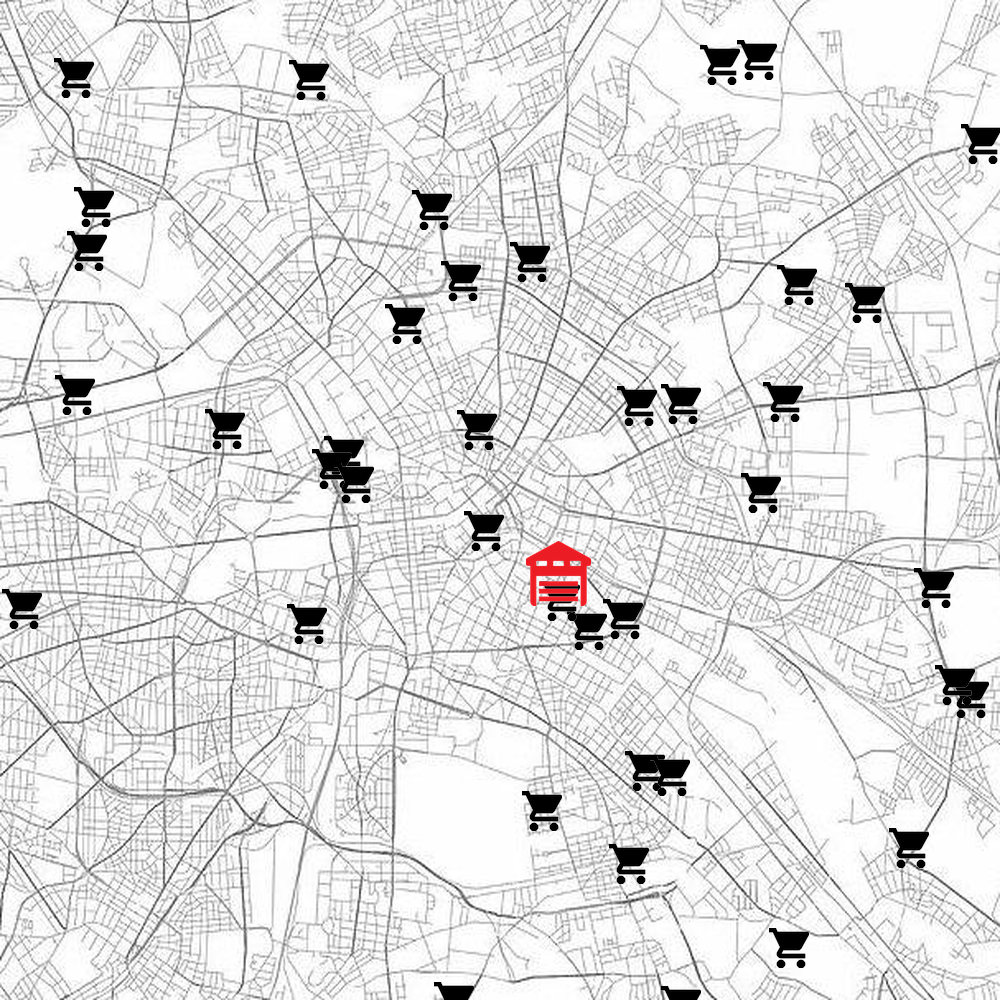
\includegraphics[width=0.95\textwidth]{pics/final2.png}
\end{subfigure}
\caption[long]{Br. magacina: 5, br. prodavnica: 40, \\cena u centru: 10000, cena inače: 5000}
\label{fig:sl2}
\end{figure}

\begin{figure}[H]
\centering
\begin{subfigure}{.5\textwidth}
    \centering
    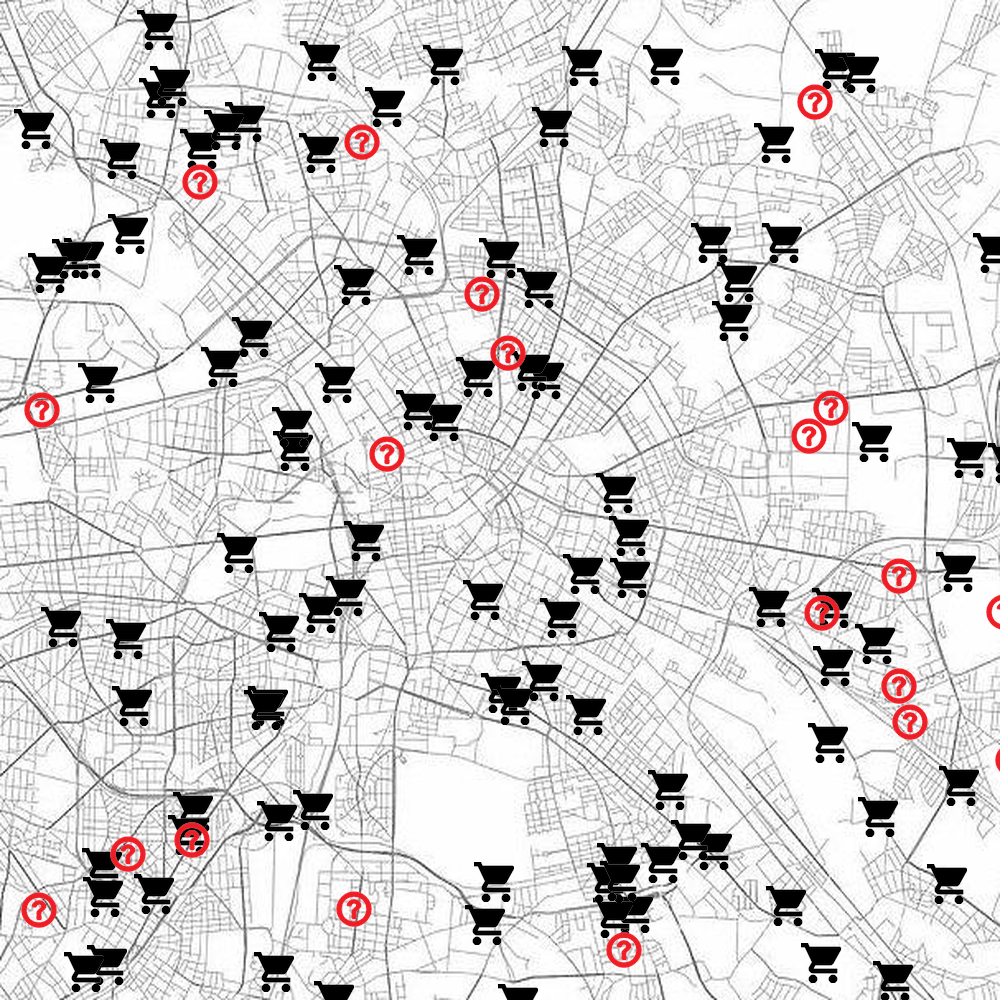
\includegraphics[width=0.95\textwidth]{pics/candidates3.png}
\end{subfigure}%
\begin{subfigure}{.5\textwidth}
    \centering
    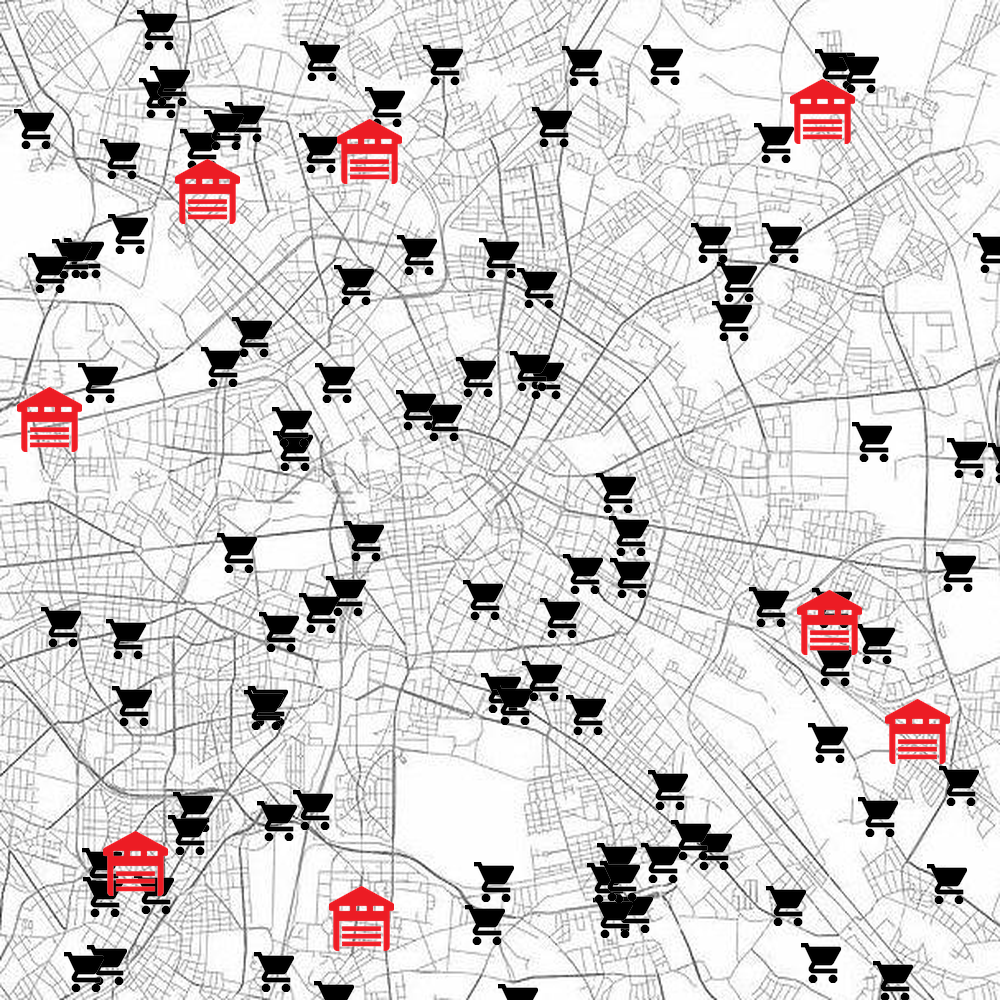
\includegraphics[width=0.95\textwidth]{pics/final3.png}
\end{subfigure}
\caption[long]{Br. magacina: 20, br. prodavnica: 100,\\ cena u centru: 10000, cena inače: 6000}
\label{fig:sl3}
\end{figure}

Vidimo da se magacini uglavnom raspoređuju ravnomerno po periferiji grada (slike 1 i 3), sem u slučaju kada jako mali broj magacina može obezbediti sve radnje (slika 2). Ovo ima smisla jedino ako je magacin u centru, jer je tada zbir udaljenosti do prodavnica najmanji, što je jeste ono što se pokazalo primerima. Inače, magacini se raspoređuju tako da je cena njihovog otvaranja manja, dakle na periferiji.

\section{Poređenje tabu pretrage sa drugim algoritmima pretrage}
Mnoge studije ispituju efikasnost i optimalnost različitih algoritama pretrage na različitim problemima. Kada je u pitanju tabu pretraga, neka istraživanja su pronašla da je ona za ispitivane probleme vidno bolja heuristika, \cite{comptabubetter} dok su druga zaključila da je kvalitet situacion i da zavisi od dimenzija i oblika problema. \cite{comptabusimilar}\cite{comptabugoodperformance} Pri tome je nekoliko istraživača došlo do zaključka da tabu pretraga često daje nešto manje optimalna rešenja sa boljom efikasnošću, dok algoritmi kao što je simulirano kaljenje daju optimalnija rešenja, ali je vreme izvršavanja duže. \cite{comptabubettertimeworseresult} Postoje i istraživanja koja tvrde da je tabu pretraga manje efikasnija od drugih algoritama. \cite{comptabuworse}\\

Iz priloženog možemo zaključiti da je teško izmeriti efikasnost metaheuristika i da ona može biti jako situaciona, ali da se tabu pretraga definitivno pokazala uporedivom sa drugim kvalitetnim tehnikama lokalne pretrage, te da se sama ili u hibridnom obliku može primeniti na mnoge probleme sa jako dobrim rezultatima.

\newpage

\section{Zaključak}
Na samom početku teksta upoznali smo se sa glavnim pojmovima i terminima bitnim za razumevanje algoritma. Dalje, prolazeći kroz njegove najbitnije karakteristike, utvrdili smo da ova metaheuristika, kao i koncept srednjeročne i dugoročne memorije pozivaju na korišćenje u rešavanju velikog broja različitih problema poznatih računarstvu. Uz navedene primere vidimo da su ideje tabu pretrage lako razumljive i jednostavne za implementaciju, pritom dajući prihvatljive, ili čak i dobre rezultate. Varijacije strategija koje bismo koristili su usko povezane sa samim problemom, te ga je potrebno podrobno razumeti i obraditi kako bi dobijeni rezultati bili što bolji. U dodatku je data relativno kratka implementacija problema N-dama u programskom jeziku Python, kako bi se čitalac podstakao na razmišljanje i dalje istraživanje praktičnih primena ovih koncepata.


\addcontentsline{toc}{section}{Literatura}
\appendix
\selectbiblanguage{serbian}
\bibliographystyle{babunsrt-lf}
\bibliography{references}

\appendix
\section{Dodatak - Testiranje parametara za N dama}
\label{appendix:a}
Kompletni rezultati urađenog testiranja se mogu naći na sledećem linku: \href{https://github.com/Min032/tabu-pretraga/blob/master/Tabu\%20dame.ipynb}{https://github.com/Min032/tabu-pretraga/blob/master/Tabu\%20dame.ipynb}

\end{document}
